%%=============================================================================
%% Proof Of Concept
%%=============================================================================
\chapter{Proof Of Concept}%
\label{ch:Proof of Concept}

In dit hoofdstuk zal er dieper ingegaan worden op de ontwikkeling van het proof-of-concept. Het uiteindelijke doel van deze proof-of-concept is om te laten zien dat het theoretisch mogelijk is om ASR-systemen stotteraars te laten verstaan met behulp van audio bewerkende functies. Op basis van de bevindingen en resultaten van het PoC kunnen er conclusies worden getrokken over de haalbaarheid van het gebruik van audio bewerkende functies om ASR-systemen stotteraars te laten verstaan.
\section{Stotter Correctie}
De eerste stap in deze proof-of-concept is het implementeren van algoritmen die het audiobestand gaan bewerken. Er worden drie algoritmen gebruikt. Het eerste algoritme is bedoeld om de verlengingen van de stotteraars te verwijderen. Daarnaast is er een algoritme dat lange pauzes van de stotteraars detecteert en verwijdert. Ten slotte is er een algoritme dat repeterende woorden uit het audiobestand verwijdert. Het doel van deze algoritmen is om de ASR-systemen een beter begrip te geven van de audiobestanden.

\subsection{Verlenging Verwijdering}

\subsection{Repetities Verwijderen}
Het algoritme voor het verwijderen van repetities start met het converteren van het audiobestand naar 22.05kHz. Dit maakt het makkelijker repetities te detecteren in de audio. Dit werd gedaan met een eenvoudige methode genaamd \emph{convert\_sr\_audio} die wordt weergegeven in figuur \ref{lst:ConvertMeth}.\\
\begin{listing}[H]
    \begin{minted}[breaklines, style=solarized-dark]{python}
        def convert_sr_audio(audio, orgSr):
        sr = 22050
        convertAudio = librosa.resample(audio, orig_sr=orgSr, target_sr=sr)
        return convertAudio
    \end{minted}
    \caption{Methode dat de audio omzet naar een frequentie van 22.05kHz.}
    \label{lst:ConvertMeth}
\end{listing}

Het volgende dat moet gebeuren, is het berekenen van de short-time energy (STE) van de audio. Dit wordt gedaan aan de hand van de volgende vergelijking:
    \[E_n = \sum_{m=-\infty}^{\infty} (x(m) w(n-m))^2 \]
Bij deze vergelijking staat $E(n)$ voor de short-time energy op tijdstip $n$. Om het concept van STE beter uit te kunnen leggen, wordt er gewerkt met een voorbeeld. In figuur \ref{fig:Signal} is een visualisatie te zien van een audiofragment, waarvoor de STE is berekend. De STE van de audio wordt weergegeven in figuur \ref{fig:STE}. Zoals te zien is in de eerste figuur, is er geen geluid aan het begin en einde van de audio, wat overeenkomt met de grafiek. Het STE van een bepaald geluid komt dus overeen met de luidheid of stilte van het geluid. Als de audio luid is op een bepaald moment, zal dit overeenkomen met een hoge energie, en als het stil is op een bepaald moment, zal dit overeenkomen met een lage energie.
\begin{figure}[H]
    \centering
    \begin{minipage}{.5\textwidth}
        \centering
        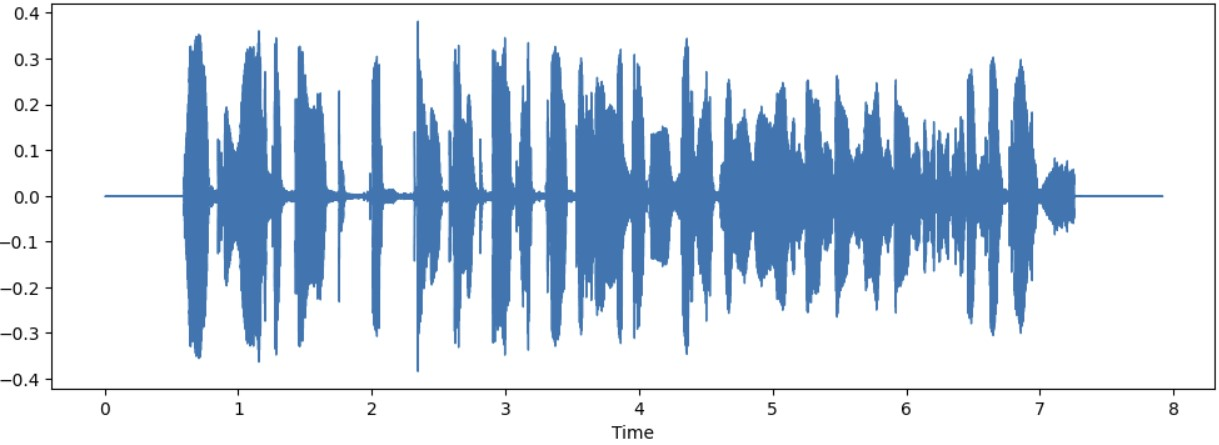
\includegraphics[width=1\linewidth]{PlotSignal}
        \captionof{figure}{Visualisatie van een audiosignaal.}
        \label{fig:Signal}
    \end{minipage}%
    \begin{minipage}{.5\textwidth}
        \centering
        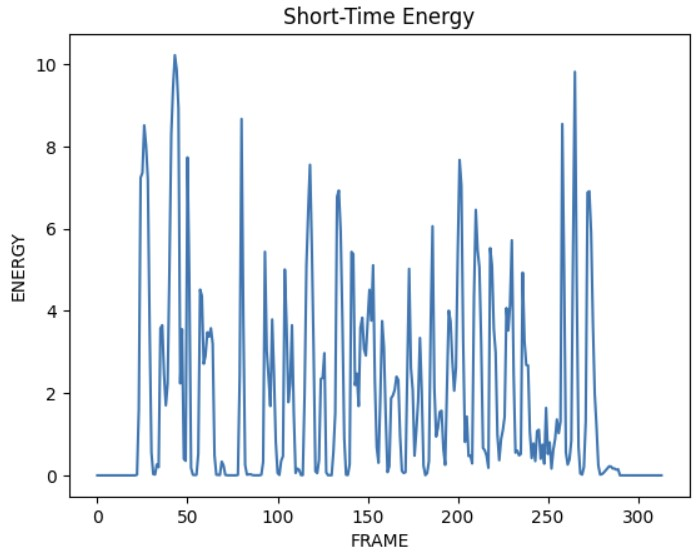
\includegraphics[width=.8\linewidth]{STESignal}
        \captionof{figure}{Short-time energy (STE) dat correspondeert met het audiosignaal dat links van deze grafiek staat.}
        \label{fig:STE}
    \end{minipage}
\end{figure}
Deze berekende energie kan dan gefilterd worden om hoge frequentie transities te verwijderen. Dit zorgt er voor dat er een dat het signaal vereffend wordt. Daarna wordt er een drempelwaarde toegepast op het vereffend signaal. De drempelwaarde die genomen werd is 0.08, dit volgt een paper waar wordt voorgesteld design voor correctie van stotter \auocite{KN2020}.
\section{Analyse}
Nu dat alle nodige algoritmen in plaats zijn en klaar voor gebruik kan er aan analyse worden gedaan. Met behulp van een methode (\ref{lst:WERMethode}) worden de datasets overlopen en getranscribeerd door de twee ASR-modellen: Whisper large-v2 en Wav2Vec 2.0 (wav2vec-large-xlsr-53-dutch). Deze methode maakt ook gebruik van de jiwer package voor het berekenen van de word error rate per model.\\

In het begin van de methode worden twee lijsten aangemaakt. De bedoeling van deze lijsten is om ze te vullen met word error rates per audio bestand. Dit wordt gedaan aan de hand van een for-lus die de dictionary in de dataset overloopt.\\

In het begin van de for-lus wordt het pad van het audiobestand bijgehouden en de transcriptie, het pad wordt als 'path' bijgehouden en de transcriptie als 'transcription'. Vervolgens wordt met behulp van het path variabele de audio ingeladen en een mel spectogram gegenereerd. Dit spectogram wordt dan benut door het Whisper model en genereert een transcriptie. Deze gegenereerde transcriptie wordt samen met de audio transcriptie gebruikt om de Word Error Rate (WER) te berekenen, waarna deze in de juiste lijst wordt opgenomen.\\

Daarna is het de beurt aan het Wav2Vec-model om een transcriptie te genereren. Hiervoor moet het pad eerst in een lege lijst worden gestoken, die dan aan het model wordt meegegeven. Waarna dit een transcriptie oplevert die direct gebruikt kan worden om de rate te calculeren. Deze rate komt dan ook terecht in de correcte lijst.\\

Wanneer de for-lus volledig is doorlopen, wordt de gemiddelde WER per model berekend met behulp van een kleine methode genaamd \emph{gemiddelde} (\ref{lst:GemMethode}). Daarnaast worden ook de twee lijsten met word error rates teruggegeven.

\begin{listing}[H]
    \begin{minted}[breaklines, style=solarized-dark]{python}
from jiwer import wer

def WERModellen(dataset):
    listWERWisper = []
    listWERWav2Vec = []
    for audio in dataset['train']:
        transcription = audio['transcription']
        path = audio['audio']['path']
        #Wisper
        audio = whisper.load_audio(path)
        audio = whisper.pad_or_trim(audio)
        mel = whisper.log_mel_spectrogram(audio).to(modelWhisper.device)
        options = whisper.DecodingOptions(fp16 = False)
        result = whisper.decode(modelWhisper, mel, options)
        rate = wer(result.text, transcription)
        listWERWisper.append(rate)
        #Wav2Vec
        path = [path]
        modelTranscr = modelWav2Vec.transcribe(path)
        transW2V = modelTranscr[0]['transcription']
        rate2 = wer(transW2V,transcription)
        listWERWav2Vec.append(rate2)
    return gemiddelde(listWERWav2Vec),gemiddelde(listWERWisper), listWERWav2Vec,listWERWisper
\end{minted}
    \caption{Methode dat de word error rate (WER) van de ASR-modellen (Whisper, Wav2Vec 2.0) berekend op een bepaalde dataset. De dataset moet als argument worden meegegeven aan de methode.}
    \label{lst:WERMethode}
\end{listing}
\begin{listing}[H]
\begin{minted}[breaklines, style=solarized-dark]{python}
def gemiddelde(listProp):
    return sum(listProp) / len(listProp)
\end{minted}
\caption{Kleinde methode om het gemiddelde te berekenen. Wordt gebruikt in de WERModellen methode om het gemiddelde WER te berekenen.}
\label{lst:GemMethode}
\end{listing}
\subsection{Zonder Audiofuncties}
Als eerste werd het gemiddelde WER op beide datasets berekend zonder enige bewerkingen te doen op de audiofragmenten. Dit wordt gedaan om te onderzoeken welk model stotterende spraak het best zou begrijpen. De hypothese bij dit onderzoek gaat als volgt: 
\begin{hyp}{0}
Beide modellen scoren dezelfde word error rates op de dataset zonder het stotteren als de dataset met het stotteren.
\end{hyp}
\begin{hyp}{1}
De modellen scoren een lagere word error rates op de dataset zonder het stotteren dan op de dataset met het stotteren.
\end{hyp}
\subsubsection{Resultaten}
Uit de gegevens blijkt dat zowel het ASR-model Wav2Vec 2.0 als het model Whisper verschillende prestaties vertonen op de datasets met en zonder stotteren. Voor de dataset met stotterende spraak had Wav2Vec 2.0 een word error rate van 0.5619\%, terwijl Whisper een word error rate van 0.3119\% behaalde. Dit suggereert dat Whisper beter in staat was om spraak van mensen met stotteren te verwerken en te transcriberen dan Wav2Vec 2.0 model.\\

Daarentegen, bij de dataset zonder stotteren presteerde beiden Wav2Vec 2.0 en Whisper beter. Wav2Vec haalde hierbij een goede WER, namelijk 0.1999\%. Whisper doet het nog een beetje beter dan het Wav2Vec model, want het haalt immers een WER van 0.1705\%.\\
\begin{figure}[H]
    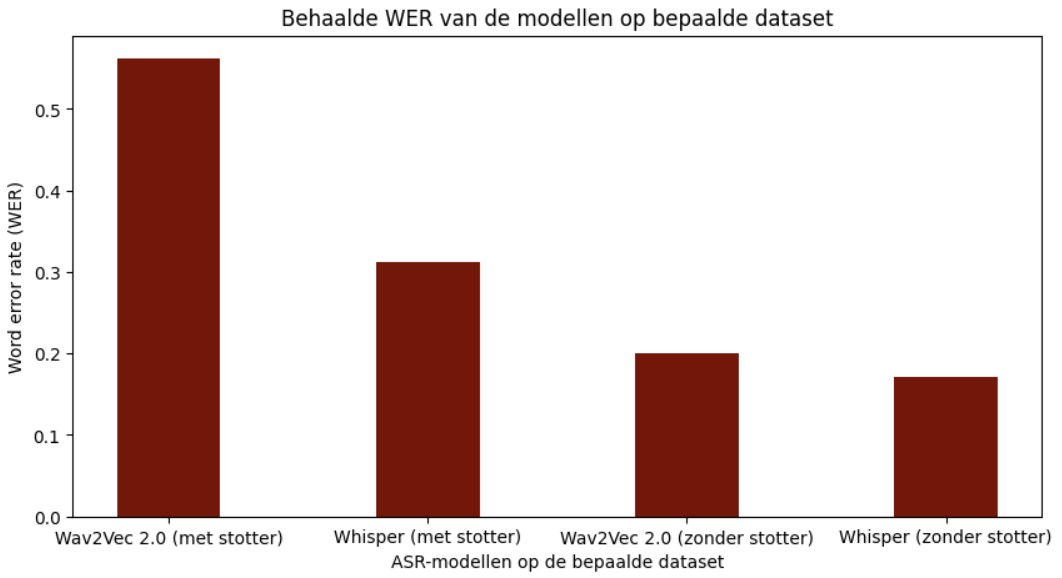
\includegraphics[scale=0.55]{BarChartDatasets}
    \caption{Staafdiagram dat de gemiddelden per dataset van de modellen weergeeft.}
    \label{fig:barchart}
\end{figure}
Beiden modellen scoren dus veel slechter op de dataset met stotterende spraak, Wav2Vec 2.0 meer dan twee maal slechter zelfs. Toch presteert Whisper nog redelijk goed in vergelijking met wat het zou kunnen behalen. Dit duidt dus op de complexiteit van spraakherkenning bij mensen met stotteren en tonen aan dat verschillende ASR-modellen uiteenlopende prestaties kunnen hebben, afhankelijk van de aard van de spraak.\\

Verder moet worden aangetoond of de nulhypothese juist is of niet. Dit kan worden gedaan met behulp van een \emph{t-test voor gepaarde steekproeven}. Deze test is gekozen omdat de gegevens in beide datasets dezelfde woorden bevatten, maar de eerste dataset stotterende spraak bevat en de tweede niet.\\

Op figuur \ref{fig:boxplot} zie je een visualisatie van de gevonden data, het toont een boxplot per dataset die de asr-modellen hebben overlopen. Nu dat we een visualisatie van de data hebben kunnen we de p-waarde berekenen. Deze waarde toont dan aan of er een significant verschil is tussen WER's op de twee datasets.
\begin{quote}
    P-waarde Whisper: 0.00294\\
    P-waarde Wav2Vec 2.0: 0.3750 * $10^{-10}$ 
\end{quote} 
Beide p-waarden duiden op een verwerping van de nullhypothese. Dit wil dus zeggen dat er een significant verschil is tussen in de word error rates van de stotter dataset en de word error rates van de dataset met normale spraak. Dit wil dus ook zeggen dat hypothese 1 correct is, beide modellen halen een lagere WER's op de normale spraak dataset.

\begin{figure}[H]
    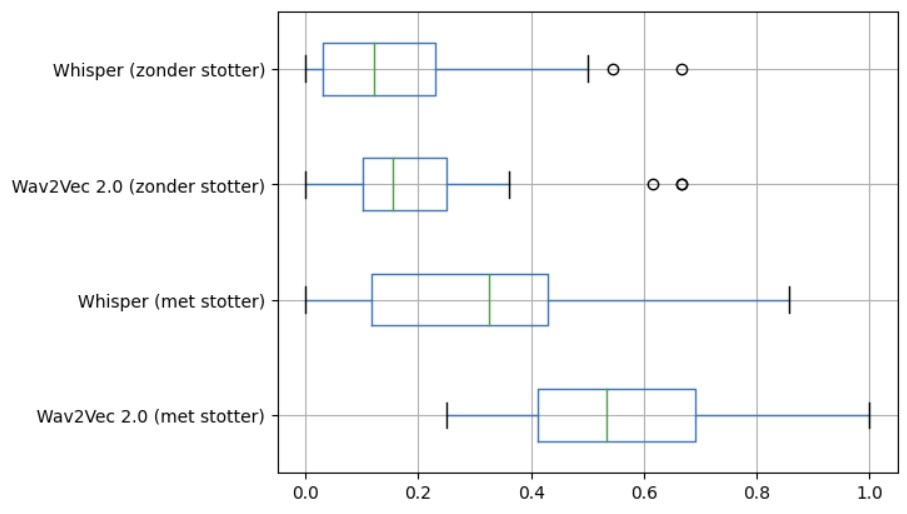
\includegraphics[scale=0.6]{BoxplotDS}
    \caption{Boxplot dat de word error rate (WER) van de audiobestanden weergeeft.}
    \label{fig:boxplot}
\end{figure}

